% !TEX TS-program = Sweave-xelatex
%!TEX encoding = UTF-8 Unicode

\documentclass[14pt]{extreport}

\usepackage{fontspec}
\newfontfamily \headingfont {Coustard}
\newfontfamily \texto {Roboto}

\usepackage{titlesec}

\titleformat{\section}{\Huge\headingfont\filcenter}{}{}{}
\titleformat{\subsection}{\Large\headingfont}
\titleformat{\subsubsection}{\large\headingfont}

\usepackage{polyglossia}

\setmainlanguage{portuges}

\usepackage{eso-pic,graphicx}
\usepackage{extsizes}
\usepackage{flowfram}
\usepackage{microtype}
\usepackage{color}
\usepackage{xcolor}

\definecolor{vermelho}{HTML}{FF9999}
\definecolor{laranja}{HTML}{FFC266}
\definecolor{verde}{HTML}{99FF99}
\definecolor{azul}{HTML}{A5C3F3}


\usepackage{tikz}

\usepackage[paperwidth=210mm, paperheight=297mm, textwidth=160mm, textheight=240mm, bindingoffset=0cm]{geometry}

\usepackage{adjustbox}

\setlength{\parskip}{1em}
\setlength{\parindent}{0cm}

\AddToShipoutPictureBG{%
  \AtPageLowerLeft{
\includegraphics[width=\paperwidth,height=\paperheight]{img/capa.jpg}}
  }

\usepackage{calc}
\newlength{\lmargin}
\setlength{\lmargin}{1in + \hoffset + \oddsidemargin}


% definição de quadro de inserção dinâmica numero das páginas
\newdynamicframe{2cm}{2cm}{\textwidth+\lmargin-2cm}{-3,4cm}[frameD-1b]
% quadro estático pensador
\newstaticframe[2]{\paperwidth}{21cm}{-\lmargin}{10cm}[frameS-1a]
\newstaticframe[4]{\paperwidth}{21cm}{-\lmargin}{-10cm}[frameS-2a]
\newstaticframe[6]{\paperwidth}{21cm}{-\lmargin}{-81mm}[frameS-3a]

% COMEÇA O DOCUMENTO! %%%%%%%%%%%%%%%%%%%%%%%%%%%%%%%%%%%%%%%%%%%%%%%%%%%%%%%%%%%%%%%%%%%%%%%%%%%%%%%%%%%%%%%%%%%%%%%%%%%%%%%%%%%%%%%%%%%%%%

\usepackage{Sweave}


\begin{document}





%\input{report-concordance}

\texto

\pagestyle{empty}
\begingroup
  \null
  \newpage
\endgroup



\ClearShipoutPicture

\begin{dynamiccontents*}{frameD-1b}
\begin{tikzpicture}
\draw(0,0) node [fill=black, minimum width=2cm, minimum height=2.1cm]{
{\sffamily\bfseries\Huge\color{white}\thepage}
};
\end{tikzpicture}
\end{dynamiccontents*}

\pagestyle{empty}

\newpage

\begin{staticcontents*}{frameS-1a}

\includegraphics[width=210mm]{img/fig1.jpg}
\end{staticcontents*}

\hfill
\vspace{100mm}

{Marcelo Tournier}, parabéns por investir na pessoa mais importante do mundo - você.

Quando nós nos conhecemos melhor, fica mais fácil de conseguirmos nossos objetivos de vida.

O Objetivo do Teste Mindset é de dar a você um Manual de Instruções de como sua mente funciona, com informações simples para que você possa melhorar os seus comportamentos, assim como a sua comunicação com amigos, colegas e familiares.

Para que este manual seja muito simples de se entender, adaptamos a linguagem de várias pesquisas sobre comportamento humano e classsificamos os comportamentos em quatro modelos mentais, que você verá na próxima página.  Quanto maior o percentual de predominância de um dos modelos no seu perfil, mais forte serão aquelas características em seu comportamento.  

Com estas informações, esperamos que você possa ser alguém melhor a cada dia.

\today.

\newpage




\section*{Qual é o seu Perfil?}



\begin{tikzpicture}
\node[midway,fill=vermelho,text width=130mm]} } };

\end{tikzpicture}

\begin{tikzpicture}
\node[fill=laranja,text width=130mm]} } };

\end{tikzpicture}

\begin{tikzpicture}
\node[fill=verde,text width=130mm]} } };

\end{tikzpicture}

\begin{tikzpicture}
\node[fill=azul,text width=130mm]} } };

\end{tikzpicture}



\newpage

\section*{Mais detalhes sobre você}



%% TESTE IF

\def\perfilprincipal{1}
\def\perfilsecundario{2}


\ifnum\perfilprincipal=1
{Marcelo Tournier}{, }{\input{txt/d1.txt}}
\fi

\ifnum\perfilprincipal=2
{Marcelo Tournier}{, }{\input{txt/i1.txt}}
\fi

\ifnum\perfilprincipal=3
{Marcelo Tournier}{, }{\input{txt/s1.txt}}
\fi

\ifnum\perfilprincipal=4
{Marcelo Tournier}{, }{\input{txt/c1.txt}}
\fi

\ifnum\perfilsecundario=1
{Além disso, }{\input{txt/d1.txt}}
\fi

\ifnum\perfilsecundario=2
{Além disso, }{\input{txt/i1.txt}}
\fi

\ifnum\perfilsecundario=3
{Além disso, }{\input{txt/s1.txt}}
\fi

\ifnum\perfilsecundario=4
{Além disso, }{\input{txt/c1.txt}}
\fi

\begin{staticcontents*}{frameS-2a}
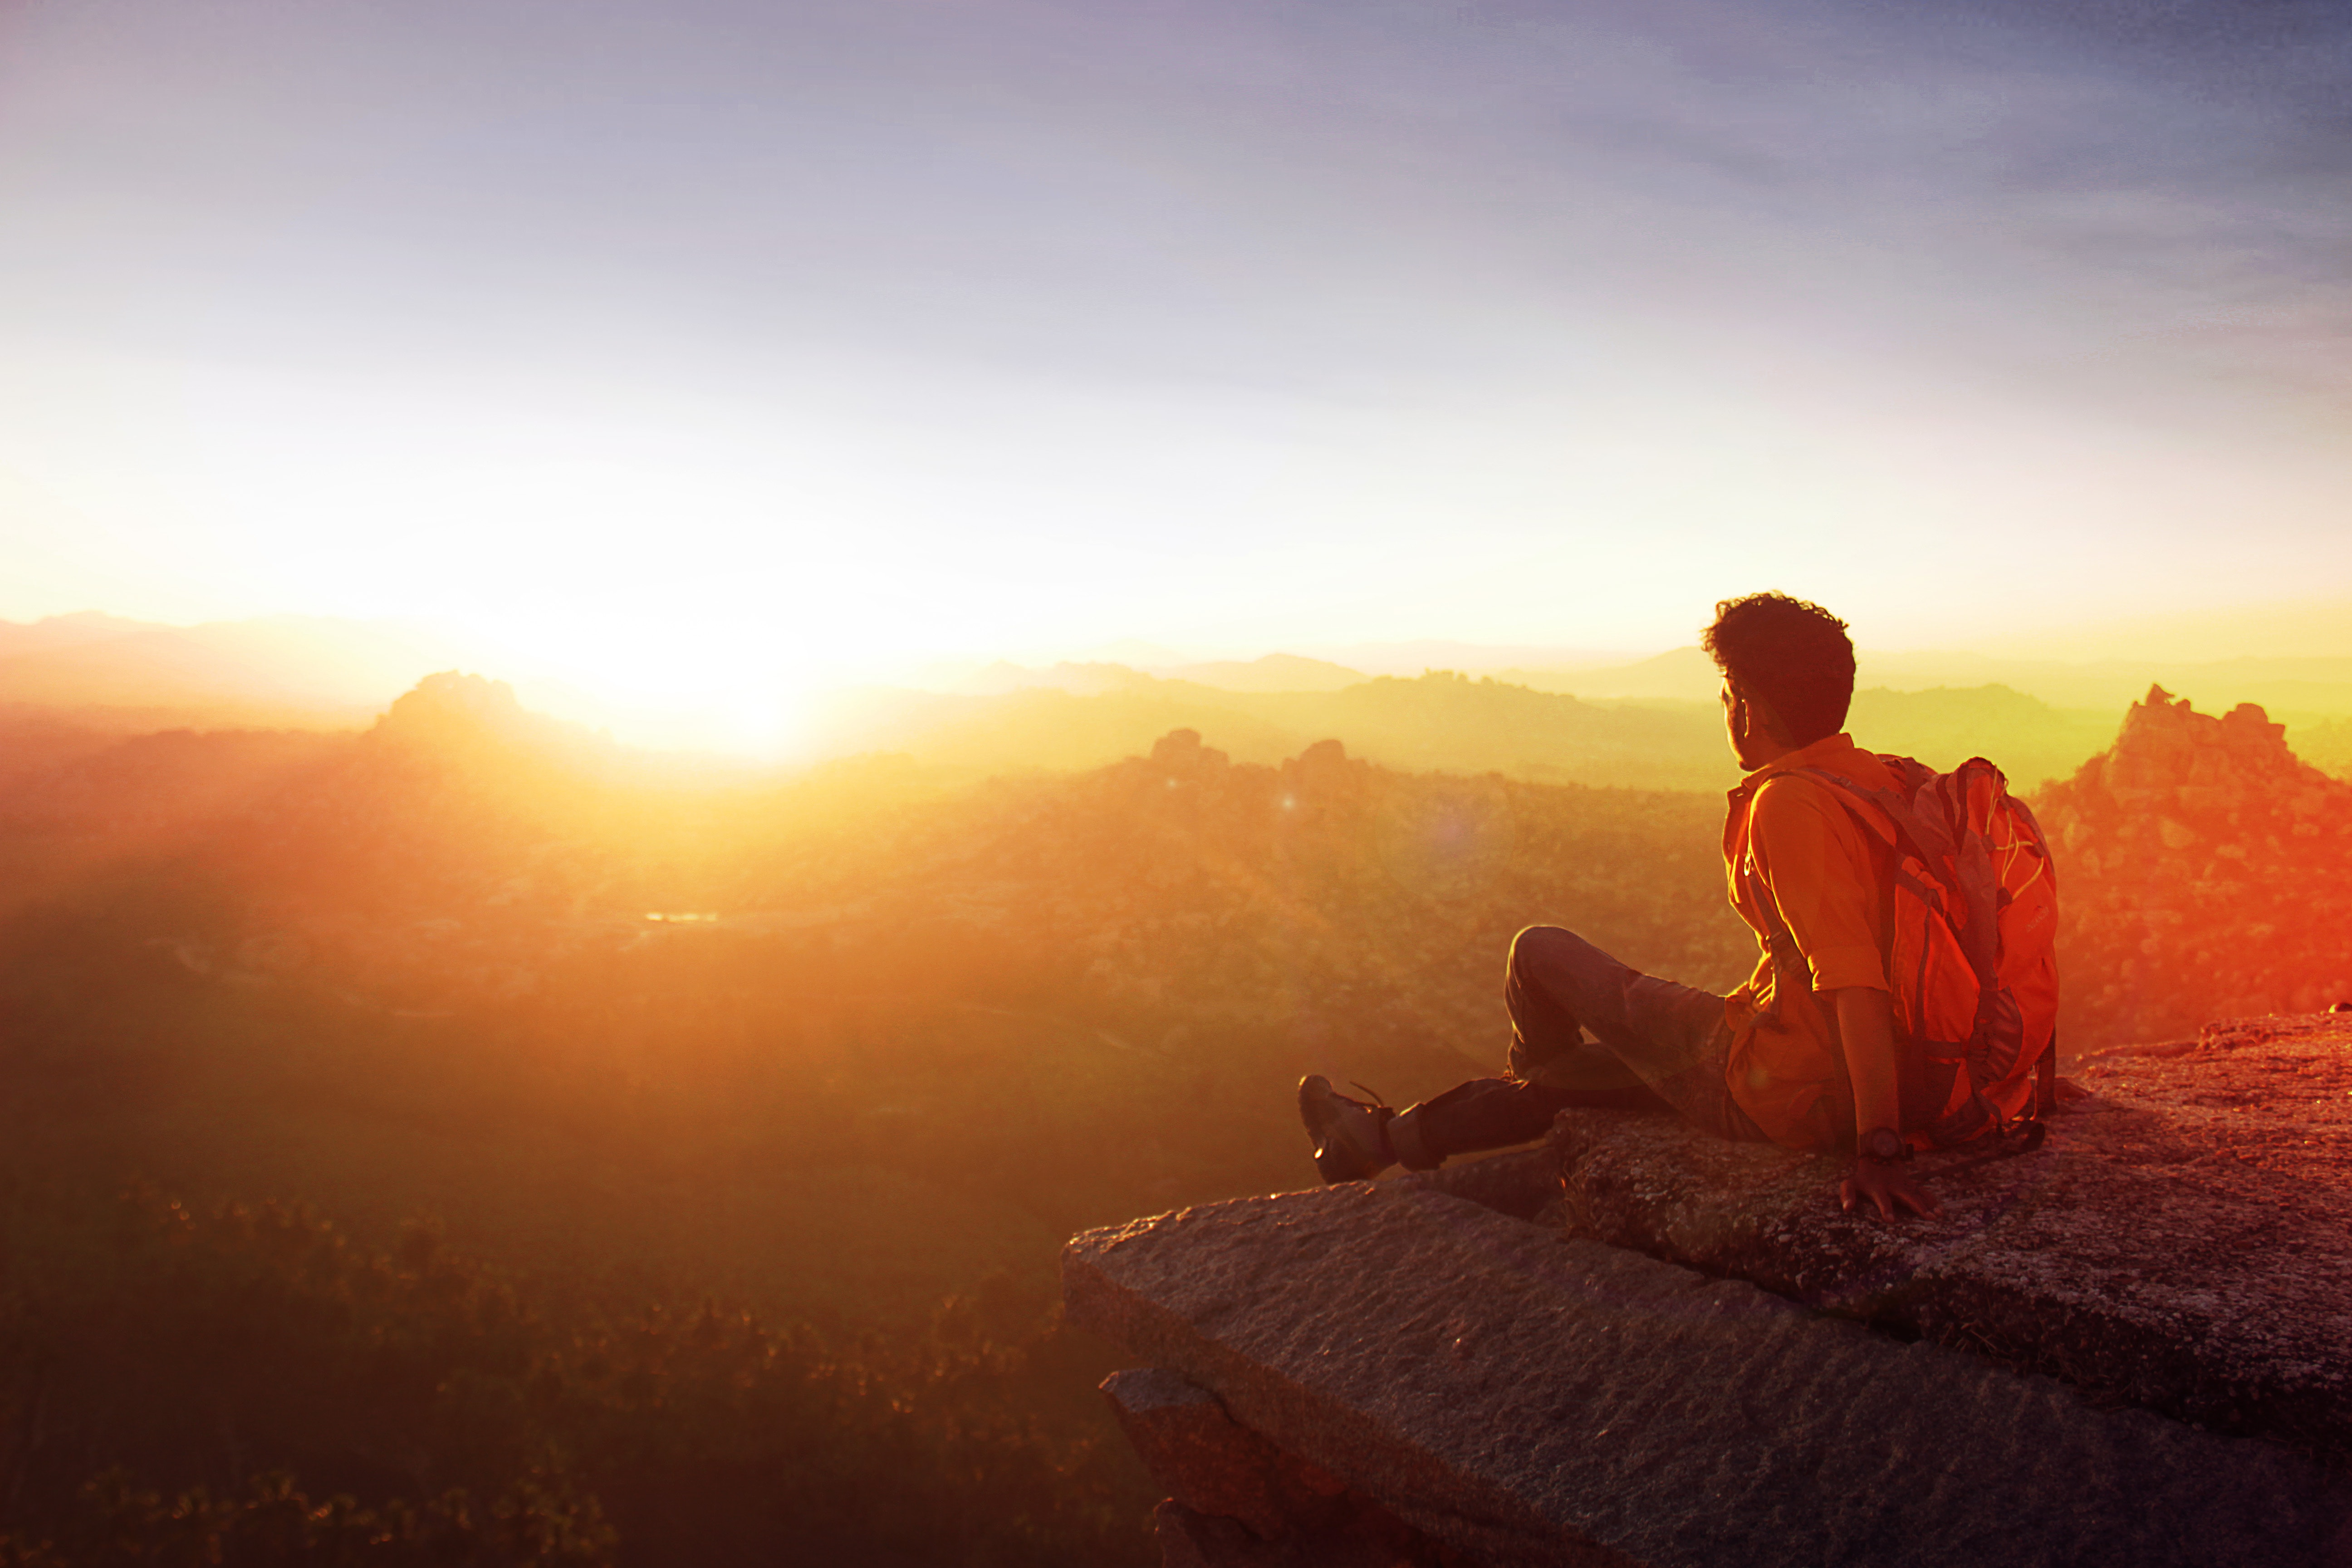
\includegraphics[width=210mm, height=105mm]{img/fig2.jpg}
\end{staticcontents*}

\newpage
% segundo bloco de conteudos
\section*{Como você pode evoluir}

\ifnum\perfilprincipal=1
{\input{txt/d2.txt}}
\fi

\ifnum\perfilprincipal=2
{\input{txt/i2.txt}}
\fi

\ifnum\perfilprincipal=3
{\input{txt/s2.txt}}
\fi

\ifnum\perfilprincipal=4
{\input{txt/c2.txt}}
\fi

\ifnum\perfilsecundario=1
{\input{txt/d2.txt}}
\fi

\ifnum\perfilsecundario=2
{\input{txt/i2.txt}}
\fi

\ifnum\perfilsecundario=3
{\input{txt/s2.txt}}
\fi

\ifnum\perfilsecundario=4
{\input{txt/c2.txt}}
\fi


%% TESTE IF

\begin{staticcontents*}{frameS-3a}

\includegraphics[width=210mm]{img/fig3.jpg}
\end{staticcontents*}

\end{document}
